%% Run LaTeX on this file several times to get Table of Contents,
%% cross-references, and citations.

\documentclass[11pt]{book}
\usepackage{gvv}
\usepackage{gvv-book-bkup}
%\usepackage{Wiley-AuthoringTemplate}
\usepackage[sectionbib,authoryear]{natbib}% for name-date citation comment the below line
%\usepackage[sectionbib,numbers]{natbib}% for numbered citation comment the above line

%%********************************************************************%%
%%       How many levels of section head would you like numbered?     %%
%% 0= no section numbers, 1= section, 2= subsection, 3= subsubsection %%
\setcounter{secnumdepth}{3}
%%********************************************************************%%
%%**********************************************************************%%
%%     How many levels of section head would you like to appear in the  %%
%%				Table of Contents?			%%
%% 0= chapter, 1= section, 2= subsection, 3= subsubsection titles.	%%
\setcounter{tocdepth}{2}
%%**********************************************************************%%
\setcounter{tocdepth}{3}
%\includeonly{ch01}
\makeindex

\begin{document}

\frontmatter
%%%%%%%%%%%%%%%%%%%%%%%%%%%%%%%%%%%%%%%%%%%%%%%%%%%%%%%%%%%%%%%%
%% Title Pages
%% Wiley will provide title and copyright page, but you can make
%% your own titlepages if you'd like anyway
%% Setting up title pages, type in the appropriate names here:

\booktitle{CBSE Math}

\subtitle{Made Simple}

\AuAff{G. V. V. Sharma}

%% \\ will start a new line.
%% You may add \affil{} for affiliation, ie,
%\authors{Robert M. Groves\\
%\affil{Universitat de les Illes Balears}
%Floyd J. Fowler, Jr.\\
%\affil{University of New Mexico}
%}

%% Print Half Title and Title Page:
%\halftitlepage
\titlepage

%%%%%%%%%%%%%%%%%%%%%%%%%%%%%%%%%%%%%%%%%%%%%%%%%%%%%%%%%%%%%%%%
%%Copyright Page

\begin{copyrightpage}{2023}
%Title, etc
\end{copyrightpage}

% Note, you must use \ to start indented lines, ie,
% 
% \begin{copyrightpage}{2004}
% Survey Methodology / Robert M. Groves . . . [et al.].
% \       p. cm.---(Wiley series in survey methodology)
% \    ``Wiley-Interscience."
% \    Includes bibliographical references and index.
% \    ISBN 0-471-48348-6 (pbk.)
% \    1. Surveys---Methodology.  2. Social 
% \  sciences---Research---Statistical methods.  I. Groves, Robert M.  II. %
% Series.\\

% HA31.2.S873 2004
% 001.4'33---dc22                                             2004044064
% \end{copyrightpage}

%%%%%%%%%%%%%%%%%%%%%%%%%%%%%%%%%%%%%%%%%%%%%%%%%%%%%%%%%%%%%%%%
%% Only Dedication (optional) 

%\dedication{To my parents}

\tableofcontents

%\listoffigures %optional
%\listoftables  %optional

%% or Contributor Page for edited books
%% before \tableofcontents

%%%%%%%%%%%%%%%%%%%%%%%%%%%%%%%%%%%%%%%%%%%%%%%%%%%%%%%%%%%%%%%%
%  Contributors Page for Edited Book
%%%%%%%%%%%%%%%%%%%%%%%%%%%%%%%%%%%%%%%%%%%%%%%%%%%%%%%%%%%%%%%%

% If your book has chapters written by different authors,
% you'll need a Contributors page.

% Use \begin{contributors}...\end{contributors} and
% then enter each author with the \name{} command, followed
% by the affiliation information.

% \begin{contributors}
% \name{Masayki Abe,} Fujitsu Laboratories Ltd., Fujitsu Limited, Atsugi, Japan
%
% \name{L. A. Akers,} Center for Solid State Electronics Research, Arizona State University, Tempe, Arizona
%
% \name{G. H. Bernstein,} Department of Electrical and Computer Engineering, University of Notre Dame, Notre Dame, South Bend, Indiana; formerly of
% Center for Solid State Electronics Research, Arizona
% State University, Tempe, Arizona 
% \end{contributors}

%%%%%%%%%%%%%%%%%%%%%%%%%%%%%%%%%%%%%%%%%%%%%%%%%%%%%%%%%%%%%%%%
% Optional Foreword:

%\begin{foreword}
%\lipsum[1-2]
%\end{foreword}

%%%%%%%%%%%%%%%%%%%%%%%%%%%%%%%%%%%%%%%%%%%%%%%%%%%%%%%%%%%%%%%%
% Optional Preface:

%\begin{preface}
%\lipsum[1-1]
%\prefaceauthor{}
%\where{place\\
% date}
%\end{preface}

% ie,
% \begin{preface}
% This is an example preface.
% \prefaceauthor{R. K. Watts}
% \where{Durham, North Carolina\\
% September, 2004}

%%%%%%%%%%%%%%%%%%%%%%%%%%%%%%%%%%%%%%%%%%%%%%%%%%%%%%%%%%%%%%%%
% Optional Acknowledgments:

%\acknowledgments
%\lipsum[1-2]
%\authorinitials{I. R. S.}  

%%%%%%%%%%%%%%%%%%%%%%%%%%%%%%%%
%% Glossary Type of Environment:

% \begin{glossary}
% \term{<term>}{<description>}
% \end{glossary}

%%%%%%%%%%%%%%%%%%%%%%%%%%%%%%%%
%\begin{acronyms}
%\acro{ASTA}{Arrivals See Time Averages}
%\acro{BHCA}{Busy Hour Call Attempts}
%\acro{BR}{Bandwidth Reservation}
%\acro{b.u.}{bandwidth unit(s)}
%\acro{CAC}{Call / Connection Admission Control}
%\acro{CBP}{Call Blocking Probability(-ies)}
%\acro{CCS}{Centum Call Seconds}
%\acro{CDTM}{Connection Dependent Threshold Model}
%\acro{CS}{Complete Sharing}
%\acro{DiffServ}{Differentiated Services}
%\acro{EMLM}{Erlang Multirate Loss Model}
%\acro{erl}{The Erlang unit of traffic-load}
%\acro{FIFO}{First in - First out}
%\acro{GB}{Global balance}
%\acro{GoS}{Grade of Service}
%\acro{ICT}{Information and Communication Technology}
%\acro{IntServ}{Integrated Services}
%\acro{IP}{Internet Protocol}
%\acro{ITU-T}{International Telecommunication Unit -- Standardization sector}
%\acro{LB}{Local balance}
%\acro{LHS}{Left hand side}
%\acro{LIFO}{Last in - First out}
%\acro{MMPP}{Markov Modulated Poisson Process}
%\acro{MPLS}{Multiple Protocol Labeling Switching}
%\acro{MRM}{Multi-Retry Model}
%\acro{MTM}{Multi-Threshold Model}
%\acro{PASTA}{Poisson Arrivals See Time Averages}
%\acro{PDF}{Probability Distribution Function}
%\acro{pdf}{probability density function}
%\acro{PFS}{Product Form Solution}
%\acro{QoS}{Quality of Service}
%\acro{r.v.}{random variable(s)}
%\acro{RED}{random early detection}
%\acro{RHS}{Right hand side}
%\acro{RLA}{Reduced Load Approximation}
%\acro{SIRO}{service in random order}
%\acro{SRM}{Single-Retry Model}
%\acro{STM}{Single-Threshold Model}
%\acro{TCP}{Transport Control Protocol}
%\acro{TH}{Threshold(s)}
%\acro{UDP}{User Datagram Protocol}
%\end{acronyms}

\setcounter{page}{1}

\begin{introduction}
This book links high school coordinate geometry to linear algebra and matrix analysis through solved problems.

\end{introduction}

\mainmatter
\chapter{Vectors}
\section{2020}
\subsection{10}
\input{2020/vetors1.0.tex}
\subsection{12}
\input{2020/vetors2.0.tex}
\section{2023}
\subsection{10}
\input{2023/vectors10-1.tex}
\input{2023/Vectors.tex}
\subsection{12}
\input{2023/vector12-1.tex}
\section{2022}
\subsection{10}
\input{2022/maths1.tex}
\subsection{12}
\begin{enumerate}

\item Write a vector of magnitude 9 units in the direction of vector \\ $-2\hat{i} + \hat{j} + 2\hat{k}$.

\item Find $\lambda$ if $\brak{2\hat{i} + 6\hat{j} + 14\hat{k}} \times \brak{\hat{i} - \lambda\hat{j} + 7\hat{k}} = \overrightarrow{0}$.

\item If $\overrightarrow{a} = \hat{i} + \hat{j} + \hat{k}$, $\overrightarrow{b} = 4\hat{i} - 2\hat{j} + 3\hat{k}$ and $\overrightarrow{c} = \hat{i} - 2\hat{j} + \hat{k}$, find a vector of magnitude 6 units which is parallel to the vector $2\overrightarrow{a} - \overrightarrow{b} + 3\overrightarrow{c}$.

\item Let $\overrightarrow{a} = \hat{i} + 4\hat{j} + 2\hat{k}$, $\overrightarrow{b} = 3\hat{i} - 2\hat{j} + 7\hat{k}$ and $\overrightarrow{c} = 2\hat{i} - \hat{j} + 4\hat{k}$. Find a vector $\overrightarrow{d}$ which is perpendicular to both $\overrightarrow{c}$ is perpendicular to both $\overrightarrow{a}$ and $\overrightarrow{b}$ and $\overrightarrow{c} \cdot \overrightarrow{d} = 18$.

\end{enumerate}
\section{2021}
\subsection{10}
\input{2021/Vectors-10.tex}
\subsection{12}
\input{2021/vectors21-12.tex}
\section{2019}
\subsection{12}
\input{2019/vectors_19.tex}
\input{2019/vect55.tex}
\input{2019/vect202.tex}
\input{2019/vect19d.tex}
\input{2019/vect203.tex}
\section{2019}
\subsection{10}
\input{2019/vecj.tex}
\section{2018}
\subsection{10}
\input{2018/vectors-CBSE.tex}
\input{2018/vec22.tex}
\subsection{12}
\input{2018/vech.tex}
\input{2018/vec6.tex}
\input{2018/vec8.tex}

\section{2017}
\subsection{10}
\input{2017/vec1.tex}
\subsection{12}
\input{2017/vec17.tex}







\section{2016}
\subsection{10}
\input{2016/vector_10.tex}
\subsection{12}
\input{2016/vector.tex}
\input{2016/VECT53.tex}

\section{2015}
\subsection{10}
\input{2015/vec5.tex}
\subsection{12}
\input{2015/vector.tex}
\section{2012}
\subsection{10}
\begin{enumerate}

\item Write a vector of magnitude 9 units in the direction of vector \\ $-2\hat{i} + \hat{j} + 2\hat{k}$.

\item Find $\lambda$ if $\brak{2\hat{i} + 6\hat{j} + 14\hat{k}} \times \brak{\hat{i} - \lambda\hat{j} + 7\hat{k}} = \overrightarrow{0}$.

\item If $\overrightarrow{a} = \hat{i} + \hat{j} + \hat{k}$, $\overrightarrow{b} = 4\hat{i} - 2\hat{j} + 3\hat{k}$ and $\overrightarrow{c} = \hat{i} - 2\hat{j} + \hat{k}$, find a vector of magnitude 6 units which is parallel to the vector $2\overrightarrow{a} - \overrightarrow{b} + 3\overrightarrow{c}$.

\item Let $\overrightarrow{a} = \hat{i} + 4\hat{j} + 2\hat{k}$, $\overrightarrow{b} = 3\hat{i} - 2\hat{j} + 7\hat{k}$ and $\overrightarrow{c} = 2\hat{i} - \hat{j} + 4\hat{k}$. Find a vector $\overrightarrow{d}$ which is perpendicular to both $\overrightarrow{c}$ is perpendicular to both $\overrightarrow{a}$ and $\overrightarrow{b}$ and $\overrightarrow{c} \cdot \overrightarrow{d} = 18$.

\end{enumerate}

\section{2010}
\subsection{12}
\begin{enumerate}

\item Write a vector of magnitude 9 units in the direction of vector \\ $-2\hat{i} + \hat{j} + 2\hat{k}$.

\item Find $\lambda$ if $\brak{2\hat{i} + 6\hat{j} + 14\hat{k}} \times \brak{\hat{i} - \lambda\hat{j} + 7\hat{k}} = \overrightarrow{0}$.

\item If $\overrightarrow{a} = \hat{i} + \hat{j} + \hat{k}$, $\overrightarrow{b} = 4\hat{i} - 2\hat{j} + 3\hat{k}$ and $\overrightarrow{c} = \hat{i} - 2\hat{j} + \hat{k}$, find a vector of magnitude 6 units which is parallel to the vector $2\overrightarrow{a} - \overrightarrow{b} + 3\overrightarrow{c}$.

\item Let $\overrightarrow{a} = \hat{i} + 4\hat{j} + 2\hat{k}$, $\overrightarrow{b} = 3\hat{i} - 2\hat{j} + 7\hat{k}$ and $\overrightarrow{c} = 2\hat{i} - \hat{j} + 4\hat{k}$. Find a vector $\overrightarrow{d}$ which is perpendicular to both $\overrightarrow{c}$ is perpendicular to both $\overrightarrow{a}$ and $\overrightarrow{b}$ and $\overrightarrow{c} \cdot \overrightarrow{d} = 18$.

\end{enumerate}



\chapter{Linear Forms}
\section{2023}
\subsection{10}
\input{2023/linear-10th.tex}
\subsection{12}                                                                                                  
\input{2023/linear-12th.tex}
\section{2022}
\subsection{10}
\input{2022/lin.tex}
\subsection{12}
\input{2022/LF.tex}
\section{2021}
\subsection{10}
\input{2021/linearforms.tex}
\subsection{12}
\input{2021/lin21.tex}
\section{2019}
\subsection{12}
\input{2019/linear_19.tex}
\input{2019/linearforms19d.tex}
\subsection{10}
\input{2019/linearj.tex}
\section{2018}
\subsection{12}
\input{2018/lineh.tex}  
\input{2018/linear6.tex} 

\section{2017}
\subsection{10}

\subsection{12}
\input{2017/liner17.tex}





\section{2016}
\subsection{12}
\input{2016/linear.tex}

\section{2015}
\subsection{12}
\input{2015/linear.tex}

\section{2011}
\subsection{10}

\begin{enumerate}
    \item The point P which divides the line segment joining the points A(2, - 5) and B(5, 2) in the ratio 2:3 lies in the quadrant
    \begin{enumerate}
        \item I
        \item II 
        \item III
        \item IV
    \end{enumerate}
    \item The mid-point of segment AB is the point P( 0, 4). If the coordinates of B are (-2, 3) then the coordinates of A are
    \begin{enumerate}
        \item (2,5)
        \item (-2,-5)
        \item (2,9)
        \item (-2,11)
    \end{enumerate}
    \item If $(3,3),(6,y),(x,7)$ and $(5,6)$ are the vertices of a parallelogram taken in order, find the values of $x$ and $y$.
    \item If two vertices of an equilateral triangle are $(3,0)$ and $(6,0)$, find the third vertex.   
    \item Find the value of $k$, if the points $P(5,4),Q(7,k)$ and $R(9,-2)$ are collinear.


\item If $A$ and $B$ are the points $(-6, 7)$ and $(-1, -5)$ respectively, then the distance $2AB$ is equal to

  \begin{enumerate}[label=(\Alph*)]
    \item $13$
    \item $26$
    \item $169$
    \item $238$
  \end{enumerate}

\item Point $P(x, 4)$ lies on the line segment joining the points $A (-5,8)$ and $B (4, -10)$. Find the ratio in which point $P$ divides the line segment $AB$. Also, find the value of $x$.

\item Find the area of the quadrilateral $ABCD$, whose vertices are $A(-3, -1)$, $B(-2, -4)$, $C(4, -1)$, and $D(3, 4)$.

\item Find the value of $y$ for which the distance between the points $A(3, -1)$ and $B(11, y)$ is $10$ units.
\end{enumerate}




\section{2010}
\subsection{12}
\input{2010/linear.tex}

\chapter{Circles}
\section{2023}
\subsection{10}
\input{2023/Circle10.tex}
\section{2022}
\subsection{12}
\input{2022/tangent1.tex}
\subsection{10}
\input{2022/circles.tex}

\section{2021}
\subsection{10}
\input{2021/circle-10.tex}
\section{2020}
\subsection{10}
\input{2020/circ10.tex}
\section{2019} 
\subsection{10}
\input{2019/cirj.tex}
\section{2018} 
\subsection{10}
\input{2018/circles-CBSE.tex}
\subsection{12}
\input{2018/cirh.tex}
\section{2017}
\subsection{10}
\input{2017/cir1.tex}



\section{2016}
\subsection{10}
\input{2016/circles_10.tex}
\subsection{12}
\input{2016/cir53.tex}

\section{2015}
\subsection{10}
\input{2015/cir5.tex}



\section{2012}
\subsection{10}
\input{2012/circles.tex}

\section{2011}
\subsection{10}

\begin{enumerate}
    \item In figure 3.60, $0$ is the centre of a circle, AB is a chord and AT is the tangent at A. If $\angle AOB = 100^\circ$, then $\angle BAT$ is equal to
    \begin{figure}[h]
        \centering
        \includegraphics{figs/circfig_1.jpg}
        \caption{}
    \end{figure}    
    \begin{enumerate}
        \item $100^\circ$
        \item $40^\circ$
        \item $50^\circ$
        \item $90^\circ$
    \end{enumerate}\newpage
    \item In figure 3.61, PA and PB are tangents to the circle with centre O. If $\angle APB=100^\circ$, then $\angle OAB$ is
    \begin{figure}[h]
        \centering
        \includegraphics{figs/circfig_2.jpg}
        \caption{}
    \end{figure}
    \begin{enumerate}
        \item $30^\circ$
        \item $60^\circ$
        \item $90^\circ$
        \item $15^\circ$
  \end{enumerate}
    \item The radii of two circles are 4cm and 3cm respectively. The diameter of the circle having area equal to the sum of the area of the two circles (in cm) is
    \begin{enumerate}
        \item 5
        \item 7 
        \item 10
        \item 14
    \end{enumerate}
    \item 	Two concentric circles are of radii $7$ cm and $r$ cm respectively, where $r>7$. A chord of the larger circle, of length $48$ cm, touches the smaller circle. Find the value of $r$.
    \item In figure 3.62, APB and CQD are semi-circles of diameter 7 cm each, while ARC and BSD are semi-circles of diameter 14 cm each. Find the perimeter of the shaded region.[Use $\pi=\dfrac{22}{7}$]
    \begin{figure}[h]
        \centering
        \includegraphics[width=5cm]{figs/circfig_3.jpg}
        \caption{}
    \end{figure}
    \item In figure 3.63, a triangle ABC is drawn to circumscribe a circle of radius 2cm such that the segments BD and DC into which BC is divided by the point of contact D are of lengths 4cm and 3cm respectively. If area of $\triangle ABC=21cm^2$, then find the lengths of sides AB and AC.
    \begin{figure}[h]
        \centering
        \includegraphics[width=4cm]{figs/circfig_4.jpg}
        \caption{}
    \end{figure}\\
    \item Find the area of the major segment $APB$, in figure 3.64, of a circle of radius $35cm$ and $\angle AOB=90^\circ$.[Use $\pi=\dfrac{22}{7}$]
     \begin{figure}[H]
        \centering
        \includegraphics[width=5cm]{figs/circfig_5.jpg}
        \caption{}
    \end{figure}
    
    \item The radii of the circular ends of a bucket of height $15$ $cm$ are $14$ $cm$ and r $cm$ ($r<14$ $cm$). If the volume of bucket is $5390$ $cm^3$, then find the value of $r$.[Use $\pi=\dfrac{22}{7}$]


\item In Figure 1, $O$ is the centre of a circle, $PQ$ is a chord, and $PT$ is the tangent at $P$. If $\angle{POQ}$=$70\degree$, then $\angle{TPQ}$ equal to
    \begin{figure}[H]
    \centering
    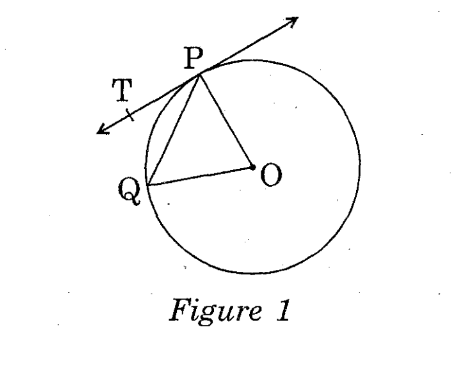
\includegraphics[width=0.8\columnwidth]{figs/figure1.jpg.png}
    \end{figure}
    \begin{enumerate}[label=(\Alph*)]
        \item $55\degree$
        \item $70\degree$
        \item $45\degree$
        \item $35\degree$
    \end{enumerate}
    
    \item In Figure $2$, $AB$ and $AC$ are tangents to the circle with center $O$ such that $\angle{BAC} = 40\degree$. Then $\angle{BOC}$ is equal to
    \begin{figure}[H]
    \centering
    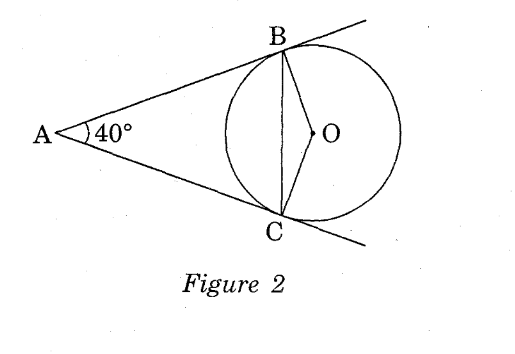
\includegraphics[width=0.8\columnwidth]{figs/figure2.jpg.png}
    \end{figure}
    \begin{enumerate}[label=(\Alph*)]
        \item $40\degree$
        \item $50\degree$
        \item $140\degree$
        \item $150\degree$
    \end{enumerate}

    \item Draw a pair of tangents to a circle of radius $3$ cm, which are inclined to each other at an angle of 60\degree.


    \item In Figure $3$, a circle touches all the four sides of whose sides are $XB = 6$ cm, $BC = 9$ cm, and $CD = 8$ cm. Find the length of side $AD$.
 \begin{figure}[H]
    \centering
    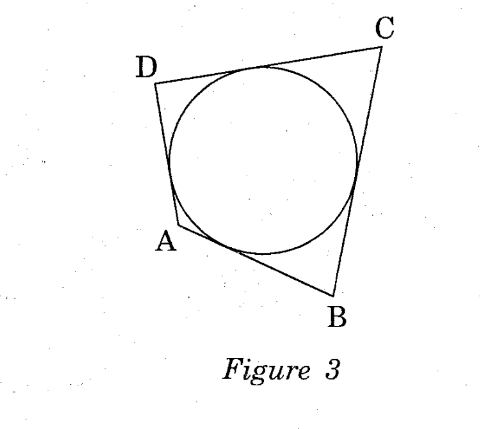
\includegraphics[width=0.8\columnwidth]{figs/figure3.jpg.png}
 \end{figure}
 
 \item Prove that the tangent at any point of a circle is perpendicular to the radius through the point of contact.
 
  

  \item A chord of a circle of radius $14$ cm subtends an angle of $120\degree $ at the center. Find the area of the corresponding minor segment of the circle. 

[Use $\pi = \dfrac{22}{7} = x$ and $\sqrt{3} = 1.73$]
\item In Figure $6$, three circles each of radius $3.5$ cm are drawn in such a way that each of them touches the other two. Find the area enclosed between these three circles (shaded region).

[Use $\pi = \dfrac{22}{7}$]
 \begin{figure}[H]
    \centering
    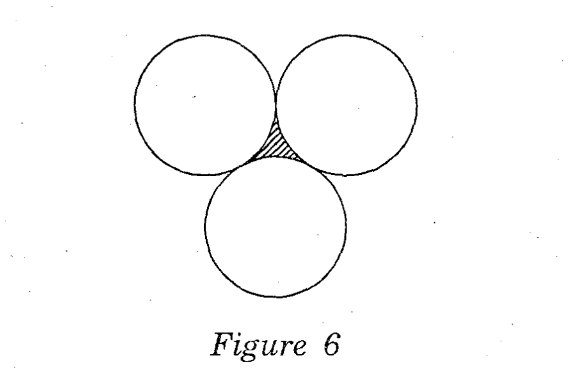
\includegraphics[width=0.8\columnwidth]{figs/figure6.jpg.png}
 \end{figure}

 \item  Find the perimeter of the shaded region in Figure $4$, if $ABCD$ is a square of side $14$ cm and $APB$ and $CPD$ are semicircles. [Use $\pi = \dfrac{22}{7}$]
\begin{figure}[H]
    \centering
    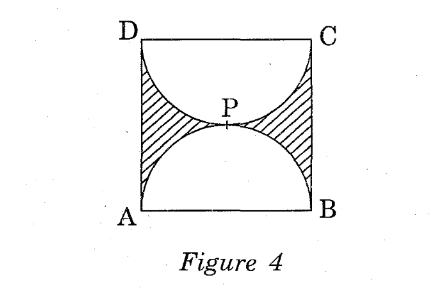
\includegraphics[width=0.8\columnwidth]{figs/figure4.jpg.png}
 \end{figure}

 \item  In Figure $5$, a triangle $PQR$ is drawn to circumscribe a circle of radius $6$ cm such that the segments $QT$ and $TR$ into which $QR$ is divided by the point of contact $T$, are of lengths $12$ cm and $9$ cm respectively. If $[PR]$, the area of $PQR$, is $40\, \text{cm}^2$, then find the lengths of sides $PQ$ and $PR$.
\begin{figure}[H]
    \centering
    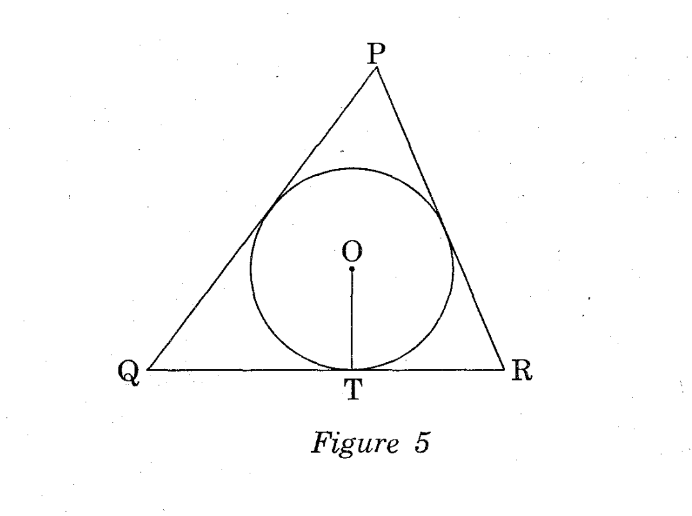
\includegraphics[width=0.8\columnwidth]{figs/figure5.jpg.png}
 \end{figure}
\end{enumerate}


\section{2010}
\subsection{12}
\input{2010/circles.tex}


\chapter{Intersection of Conics}
\section{2022}
\input{2022/chords.tex}
\section{2021}
\subsection{12}
\input{2021/con21.tex}
\section{2019}
\subsection{12}
\input{2019/intersection_19.tex}
\input{2019/inter55.tex}
\section{2018}
\subsection{12}
\input{2018/intersec6.tex}
\input{2018/intco8.tex}
\section{2010}
\subsection{12}
\input{2010/intersec.tex}





\chapter{Probability}
\section{2021}
\subsection{10}
\input{2021/probability.tex}
\subsection{12}
\input{2021/probability_cbse_21.tex}
\section{2023}
\subsection{10}
\begin{enumerate}

\item A family has 2 children. Find the probability that both are boys if it is known that
    \begin{enumerate}
        \item at least one of the children is a boy
        \item the elder child is a boy
    \end{enumerate}

\item A box contains 4 balls. Two balls are drawn at random, and are found to be white. What is the probability that all balls are white.

\end{enumerate}
\subsection{12}
\input{2023/probability12.tex}
\section{2022}
\subsection{10}
\input{2022/probability10.tex}
\section{2022}
\subsection{12}
\input{2022/probability.tex}
\section{2020}
\subsection{10}
\input{2020/prob10.tex}
\subsection{12}
\input{2020/prob12.tex}
\section{2019}
\subsection{12}
\input{2019/probab_19.tex}
\input{2019/probb55.tex}
\input{2019/prob202.tex}
\input{2019/probab19d.tex}
\input{2019/prob203.tex}
\section{2019}
\subsection{10}
\input{2019/probj.tex}
\section{2018}
\subsection{10}
\input{2018/probability-CBSE.tex}
\input{2018/prob22.tex}
\subsection{12}
\input{2018/probh.tex}
\input{2018/prob6.tex}
\input{2018/pro8.tex}

\section{2017}
\subsection{10}
\input{2017/prob1.tex}
\subsection{12}
\input{2017/prob17.tex}




\section{2016}
\subsection{10}
\input{2016/prob_10.tex}
\subsection{12}
\begin{enumerate}

\item A family has 2 children. Find the probability that both are boys if it is known that
    \begin{enumerate}
        \item at least one of the children is a boy
        \item the elder child is a boy
    \end{enumerate}

\item A box contains 4 balls. Two balls are drawn at random, and are found to be white. What is the probability that all balls are white.

\end{enumerate}
\input{2016/PROB53.tex}
\section{2015}
\subsection{10}
\begin{enumerate}

\item A family has 2 children. Find the probability that both are boys if it is known that
    \begin{enumerate}
        \item at least one of the children is a boy
        \item the elder child is a boy
    \end{enumerate}

\item A box contains 4 balls. Two balls are drawn at random, and are found to be white. What is the probability that all balls are white.

\end{enumerate}
\input{2015/prob5.tex}
\subsection{12}
\input{2015/probab.tex}
\section{2012}
\subsection{10}
\input{2012/probability.tex}

\section{2011}
\subsection{10}

\begin{enumerate}
    \item Which of the following cannot be the probability of an event?
    \begin{enumerate}
        \item 1.5
        \item $\dfrac{3}{5}$
        \item $25\%$
        \item 0.3
    \end{enumerate}
    \item A coin is tossed two times. Find the probability of getting at least one head.
    \item Two dice are rolled once. Find the probability of getting such numbers on two dice, whose product is a perfect square.
    \item A game consists of tossing a coin 3 times and noting its outcome each time. Hanif wins if he gets three heads or three tails, and loses otherwise. Calculate the probability that Hanif will lose the game.


\item A card is drawn from a well-shuffled deck of $52$ playing cards. The probability that the card will not be an ace is

\begin{enumerate}[label=(\Alph*)]
    \item $\dfrac{1}{13}$
    \item $\dfrac{1}{4}$
    \item $\dfrac{12}{13}$
    \item $\dfrac{3}{4}$
\end{enumerate}

A box contains 80 discs which are numbered from $1$ to $80$. If one disc is drawn at random from the box, find the probability that it bears a perfect square number.

\item Two dice are rolled once. Find the probability of getting such numbers on the two dice, whose product is $12$.


\item A ticket is drawn at random from a bag containing tickets numbered from $1$ to $40$. Find the probability that the selected ticket has a number which is a multiple of $5$.
\end{enumerate}



\section{2010}
\subsection{12}
\begin{enumerate}

\item A family has 2 children. Find the probability that both are boys if it is known that
    \begin{enumerate}
        \item at least one of the children is a boy
        \item the elder child is a boy
    \end{enumerate}

\item A box contains 4 balls. Two balls are drawn at random, and are found to be white. What is the probability that all balls are white.

\end{enumerate}

\chapter{Construction}
\section{2023}
\subsection{10}
\input{2023/construction-10th.tex}
\section{2022}
\subsection{10}
\input{2022/construction.tex}
\section{2021}
\subsection{10}
\input{2021/construction.tex}
\section{2020}
\subsection{10}
\input{2020/cont.tex}
\section{2019} 
\subsection{10}
\input{2019/consj.tex}
\section{2018} 
\subsection{10}
\input{2018/construction-CBSE.tex}
\input{2018/con22.tex}
\section{2017}
\subsection{10}
\input{2017/cons1.tex}





\section{2016}
\subsection{10}
\input{2016/construction_10.tex}
\section{2015}
\subsection{10}
\input{2015/construction.tex}
\input{2015/con5.tex}
\section{2012}
\subsection{10}
\input{2012/construction.tex}

\section{2011}
\subsection{10}
\input{2011/construction_psv.tex}

\section{2010}
\subsection{12}
\input{2010/construction.tex}


\chapter{Optimization}
\section{2023}
\input{2023/opti.tex}
\section{2021}
\subsection{12}
\input{2022/opt_vect.tex}
\section{2022}
\subsection{12}
\input{2021/opti-21-12.tex}
\section{2020}
\subsection{12}
\input{2020/Assignment2.tex}
\section{2019}
\subsection{12}
\input{2019/opti_19.tex}
\input{2019/opt55.tex}
\input{2019/opti202.tex}
\input{2019/opti203.tex}
\section{2018}
\subsection{10}
\input {2018/opt22.tex}
\subsection{12}
\input{2018/opth.tex}
\input{2018/opti6.tex}
\input{2018/opt8.tex}

\section{2017}
\subsection{10}

\subsection{12}
\input{2017/opt17.tex}




\section{2016}
\subsection{12}
\begin{enumerate}

\item One kind of cake requires 300g of flour and 15g of fat, another kind of cake requires 150g of flour and 30g of fat. Find the maximum number of cakes which can be made from 7.5kg of flour and 600g of fat, assuming that there is no shortage of the other ingredients used in making the cakes. Make it as an LPP and solve it graphically.

\end{enumerate}
\input{2016/OPTI53.tex}

\section{2015}
\subsection{12}
\begin{enumerate}

\item One kind of cake requires 300g of flour and 15g of fat, another kind of cake requires 150g of flour and 30g of fat. Find the maximum number of cakes which can be made from 7.5kg of flour and 600g of fat, assuming that there is no shortage of the other ingredients used in making the cakes. Make it as an LPP and solve it graphically.

\end{enumerate}

\section{2010}
\subsection{12}
\begin{enumerate}

\item One kind of cake requires 300g of flour and 15g of fat, another kind of cake requires 150g of flour and 30g of fat. Find the maximum number of cakes which can be made from 7.5kg of flour and 600g of fat, assuming that there is no shortage of the other ingredients used in making the cakes. Make it as an LPP and solve it graphically.

\end{enumerate}


\chapter{Algebra}
\section{2020}
\subsection{10}
\input{2020/ALGEBRA-CBSE-10.tex}
\section{2020}
\subsection{12}
\input{2020/ALGEBRA-CBSE-12.tex}
\section{2023}
\subsection{10}
\input{2023/algebra.tex}
\section{2022}
\subsection{10}
\input{2022/algebra.tex}
\section{2021}
\subsection{10}
\input{2021/algebra.tex}
\input{2021/algebra2021.tex}

\section{2021}
\subsection{12}
\input{2021/Algebra12.tex}

\section{2019}
\subsection{12}
\input{2019/algeb_19.tex}
\input{2019/alger55.tex}
\input{2019/Alg203.tex}
\section{2019} 
\subsection{10}
\input{2019/algebj.tex}
\section{2018} 
\subsection{10}
\input{2018/Algebra-CBSE.tex}
\input{2018/alg22.tex}
\subsection{12}
\input{2018/algh.tex}
\input{2018/alge6.tex}
\input{2018/al8.tex}

\section{2017}
\subsection{10}
\input{2017/alge1.tex}
\subsection{12}
\input{2017/alg17.tex}



\section{2016}
\subsection{10}
\input{2016/alg_10.tex}
\subsection{12}
\input{2016/algebra.tex}
\input{2016/alg53.tex}
\section{2015}
\subsection{10}
\input{2015/algebra.tex}
\input{2015/alg5.tex}
\subsection{12}
\input{2015/alg.tex}
\section{2012}
\subsection{10}
\input{2012/algebra.tex}

\section{2011}
\subsection{10}
\begin{enumerate}
    \item The roots of the equation constant, are $x^2+x-p\brak{p+1}=0$, where p is a constant,are
        \begin{enumerate}
            \item $p,\brak{p+1}$
            \item $-p,\brak{p+1}$
            \item $p,-\brak{p+1}$
            \item $-p,-\brak{p+1}$
        \end{enumerate}
    \item Find the value of $p$ so that the quadratic equation $px\brak{x-3}+9=0$ has two equal roots.
    \item Find the roots of the following quadratic equation:\[2\sqrt{3}x^2-5x+\sqrt{3}=0\]
    \item A motor boat whose speed is $20$$km/h$ in still water, takes 1 hour more to go 48 km upstream than to return downstream to the same spot. Find the speed of the stream.    
    \item Find the roots of the equation \[\dfrac{1}{x+4}-\dfrac{1}{x-7}=\dfrac{11}{30}, x\neq -4,7\] 
    \item The roots of the equation $x^3 - 3x - \brak{m(m + 3)} = 0$, where $m$ is a constant, are:

    \begin{enumerate}[label=(\Alph*)]
        \item $m, m + 3$
        \item $-m, m + 3$
        \item $m, -(m + 3)$
        \item $-m, -(m + 3)$
    \end{enumerate}
    \item The roots of the equation $x^3 - 3x - \brak{m(m + 3)} = 0$, where $m$ is a constant, are:

    \begin{enumerate}[label=(\Alph*)]
        \item $m, m + 3$
        \item $-m, m + 3$
        \item $m, -(m + 3)$
        \item $-m, -(m + 3)$
    \end{enumerate}
    
\item Find the value of $m$ so that the quadratic equation $mx^2 = 6t + (L - x)$ has two equal roots.     
         
\item Find the roots of the following quadratic equation: $x^2 - 3\sqrt{5} \cdot x + 10 = 0$. 

Find the roots of the equation $\dfrac{1}{2x-3} + \dfrac{1}{x-5} = 1$, where $x \neq \dfrac{3}{2}, 5$.



\begin{enumerate}[label=(\Alph*)]
    \item $m, m + 3$
    \item $-m, m + 3$
    \item $m, -(m + 3)$
    \item $-m, -(m + 3)$
\end{enumerate}
\item The roots of the equation $x^3 - 3x - \brak{m(m + 3)} = 0$, where $m$ is a constant, are:

\begin{enumerate}[label=(\Alph*)]
    \item $m, m + 3$
    \item $-m, m + 3$
    \item $m, -(m + 3)$
    \item $-m, -(m + 3)$
\end{enumerate}

\item Find the value of $m$ so that the quadratic equation $mx^2 = 6t + (L - x)$ has two equal roots.     
     
\item Find the roots of the following quadratic equation: $x^2 - 3\sqrt{5} \cdot x + 10 = 0$. 

\item Find the roots of the equation $\dfrac{1}{2x-3} + \dfrac{1}{x-5} = 1$, where $x \neq \dfrac{3}{2}, 5$.
\end{enumerate}


\section{2010}
\subsection{12}
\input{2010/algebra.tex}

\chapter{Geometry}
\section{2023}
\subsection{10}
\input{2023/ASSIGNMENT_1.tex}
\input{2023/latexwork.tex}
\section{2022}
\subsection{10}
\input{2022/latex.tex}

\section{2021}
\subsection{10}
\input{2021/geometry2021.tex}
\section{2020}
\subsection{10}
\input{2020/Gupdates_10.tex}
\section{2019}
\subsection{10}
\input{2019/geoj.tex}
\section{2018}
\subsection{10}
\input{2018/Geometry-CBSE.tex}
\input{2018/geo22.tex}
\subsection{12}
\input{2018/geoh.tex}
\input{2018/geo6.tex}

\section{2017}
\subsection{10}
\input{2017/geo1.tex}
\subsection{12}
\input{2017/geom17.tex}



\section{2016}
\subsection{10}
\input{2016/geometry_10.tex}
\subsection{12}
\input{2016/Geometry.tex}
\input{2016/GEO53.tex}
\section{2015}
\subsection{10}
\begin{enumerate}

\item Write the distance of the following plane from the origin:
    \begin{align*}
    2x - y + 2z + 1 = 0
    \end{align*}

\item Find the points on the line $\frac{x+2}{3} = \frac{y+1}{2} = \frac{z-3}{2}$ at a distance of 5 units from the point $P\brak{1, 3, 3}$.

\item Find the distance of the point $P\brak{6, 5, 9}$ from the plane determined by the points $A\brak{3, -1, 2}$, $B\brak{5, 2, 4}$ and $C\brak{-1, -1, 6}$.

\item Find the coordinates of the foot of the perpendicular and the perpendicular distance of the point $P\brak{3, 2, 1}$ from the plane $2x - y + z + 1 = 0$. Find also, the image of the point in the plane.

\item Find the area of the circle $4x^2 + 4y^2 = 9$ which is interior to the parabola $x^2 = 4y$.

\item Using integration, find the area of the triangle ABD, coordinates of whose vertices are A(4, 1), B(6, 6) and C(8, 4).

\end{enumerate}
\input{2015/geo5.tex}
\section{2012}
\subsection{10}
\begin{enumerate}

\item Write the distance of the following plane from the origin:
    \begin{align*}
    2x - y + 2z + 1 = 0
    \end{align*}

\item Find the points on the line $\frac{x+2}{3} = \frac{y+1}{2} = \frac{z-3}{2}$ at a distance of 5 units from the point $P\brak{1, 3, 3}$.

\item Find the distance of the point $P\brak{6, 5, 9}$ from the plane determined by the points $A\brak{3, -1, 2}$, $B\brak{5, 2, 4}$ and $C\brak{-1, -1, 6}$.

\item Find the coordinates of the foot of the perpendicular and the perpendicular distance of the point $P\brak{3, 2, 1}$ from the plane $2x - y + z + 1 = 0$. Find also, the image of the point in the plane.

\item Find the area of the circle $4x^2 + 4y^2 = 9$ which is interior to the parabola $x^2 = 4y$.

\item Using integration, find the area of the triangle ABD, coordinates of whose vertices are A(4, 1), B(6, 6) and C(8, 4).

\end{enumerate}
%\input{2023/gouthami.tex}
%\input{2023/algebra-10.tex}
%\subsection{10}
%\input{2023/bindhu.tex}
\section{2011}
\subsection{10}
\begin{enumerate}
    \item A sphere of diameter 18 cm is dropped into a cylindrical vessel of diameter 36 cm, partly filled with water. If the sphere is completely submerged, then the water level rises (in cm) by
    \begin{enumerate}
        \item 3
        \item 4 
        \item 5
        \item 6
    \end{enumerate}
    \item Two cubes, each of side 4 cm are joined end to end. Find the surface area of the resulting cuboid.
    \item Find that value(s) of x for which the distance between the points $P(x,4)$ and $Q(9,10)$ is $10$units.
    \item From a solid cylinder whose height is 15 cm and diameter 16 cm, a conical cavity of the same height and same diameter is hollowed out. Find the total surface area of the remaining solid. [Take $n=3.14$]


\item The perimeter $\brak{in\,cm}$ of a square circumscribing a circle of radius $a$ cm, is  
\begin{enumerate}[label=(\Alph*)]
    \item $8a$
    \item $4a$
    \item $2a$
    \item $16a$
\end{enumerate}
\item The radius $\brak{in\,cm}$ of the largest right circular cone that can be cut out from a cube of edge $4.2$ cm is

\begin{enumerate}[label=(\Alph*)]
\item $4.2$
\item $2.1$
\item $8.4$
\item $1.05$
\end{enumerate}

\item An open metal bucket is in the shape of a frustum of a cone of height $21$ cm with radii of its lower and upper ends as $10$ cm and $20$ cm at Rs. $30$ per liter. Find the cost of milk which can completely fill the bucket at Rs $30$ per liter. 

[Use $\pi = \dfrac{22}{7}$]

\item Find the area of the triangle formed by joining the mid-points of the sides of the triangle whose vertices are $A(2, 1)$, $B(4, 3)$, and $C(2, 5)$.


\item Two cubes each of volume 27 ${cm}^3$ are joined end to end to form a solid. Find the surface area of the resulting cuboid.

\item A cone of height $20$ cm and radius of base $5$ cm is made up of modelling clay. A child reshapes it in the form of a sphere. Find the diameter of the sphere.

\item Water is flowing at the rate of $15$ km/hour through a pipe of diameter $14$ cm into a cuboidal pond which is $50$ m long and $44$ m wide. In what time will the level of water in the pond rise by $21$ cm?


\item A train travels $180$ km at a uniform speed. If the speed had been $9$ km/hour more, it would have taken $1$ hour less for the same journey. Find the speed of the train.
\end{enumerate}

\section{2010}
\subsection{12}
\begin{enumerate}

\item Write the distance of the following plane from the origin:
    \begin{align*}
    2x - y + 2z + 1 = 0
    \end{align*}

\item Find the points on the line $\frac{x+2}{3} = \frac{y+1}{2} = \frac{z-3}{2}$ at a distance of 5 units from the point $P\brak{1, 3, 3}$.

\item Find the distance of the point $P\brak{6, 5, 9}$ from the plane determined by the points $A\brak{3, -1, 2}$, $B\brak{5, 2, 4}$ and $C\brak{-1, -1, 6}$.

\item Find the coordinates of the foot of the perpendicular and the perpendicular distance of the point $P\brak{3, 2, 1}$ from the plane $2x - y + z + 1 = 0$. Find also, the image of the point in the plane.

\item Find the area of the circle $4x^2 + 4y^2 = 9$ which is interior to the parabola $x^2 = 4y$.

\item Using integration, find the area of the triangle ABD, coordinates of whose vertices are A(4, 1), B(6, 6) and C(8, 4).

\end{enumerate}

\chapter{Discrete}
\section{2022}
\subsection{10}
\input{2022/discrete.tex}
\section{2023}
\subsection{10}
\input{2023/firstlatex.tex}
\section{2021}
\subsection{10}
\input{2021/discrete_21.tex}
\section{2020}
\subsection{10}
\input{2020/dist.tex}
\section{2019}
\subsection{10}
\input{2019/dissj.tex}
\section{2018}
\subsection{10}
\input{2018/discrete-CBSE.tex}
\subsection{12}
\input{2018/dish.tex}
\section{2017}
\subsection{10}
\input{2017/dis1.tex}



\section{2016}
\subsection{10}
\input{2016/discrete_10.tex}
\section{2015}
\subsection{10}
\input{2015/dis5.tex}

%\subsection{12}
%\input{2016/Geometry.tex}
\section{2012}
\subsection{10}
\input{2012/discrete.tex}
\section{2011}
\subsection{10}
\input{2011/discrete_psv.tex}
\section{2010}
\subsection{12}
\input{2010/discrete.tex}

\chapter{Number Systems}
\section{2019}
\subsection{10}
\input{2019/numsysj.tex}
\section{2018}
\subsection{10}
\input{2018/num22.tex}
\section{2012}
\subsection{10}
\input{2012/number_sys.tex}
\section{2011}
\subsection{10}
\begin{enumerate}
\item Find how many two-digit numbers are divisible by $6$.
 How many multiples of $4$ lie between $10$ and $250$ ? Also find their sum.
  

\item If $P\left(\dfrac{a}{2},4\right)$ is the midpoint of the line-segment joining the points $A(-6, 5)$ and $B(-2, 3)$, then the value of $a$ is

\begin{enumerate}[label=(\Alph*)]
    \item $-8$
    \item $3$
    \item $-4$
    \item $4$
\end{enumerate}
\item Draw a line segment $AB$ of length $7$ cm. Using ruler and compasses, find a point $P$ on $AB$ such that $\dfrac{AP}{AB} = \dfrac{3}{5}$.
\end{enumerate}

\section{2010}
\subsection{12}
\input{2010/numbersys.tex}


\chapter{Differentiation}
\section{2023}
\subsection{12}
\input{2023/differentiation.tex}

\section{2022}
\subsection{12}
\input{2022/maths.tex}
\section{2021}
\subsection{10}
\begin{enumerate}

\item Solve the following differential equation:
    \begin{align*}
    \brak{x^2 - 1}\frac{dy}{dx} + 2xy = \frac{1}{x^2 - 1}; \lvert x \rvert \neq 1
    \end{align*}

\item Solve the following differential equation:
    \begin{align*}
    \sqrt{1 + x^2 + y^2 + x^2 y^2} + xy\frac{dy}{dx}= 0
    \end{align*}

\item Show that the differential equation
    $
    \brak{x-y}\frac{dy}{dx} = x + 2y
    $
    is homogenous and solve it.

    \item If $y = e^{a\sin^{-1} x}$, $-1 \le x \le 1$, then show that
    \begin{align*}
    \brak{1 - x^2}\frac{d^2y}{dx^2} - x\frac{dy}{dx} - a^2y = 0
    \end{align*}

\item If $y = \cos^{-1} \brak{\frac{3x + 4 \sqrt{1 - x^2}}{5}}$, find $\frac{dy}{dx}$.

\end{enumerate}
\section{2021}
\subsection{12}
\input{2021/diffn.tex}
\section{2021}
\subsection{12}
\input{2021/differ.tex}
\section{2020}
\subsection{12}
\begin{enumerate}

\item Solve the following differential equation:
    \begin{align*}
    \brak{x^2 - 1}\frac{dy}{dx} + 2xy = \frac{1}{x^2 - 1}; \lvert x \rvert \neq 1
    \end{align*}

\item Solve the following differential equation:
    \begin{align*}
    \sqrt{1 + x^2 + y^2 + x^2 y^2} + xy\frac{dy}{dx}= 0
    \end{align*}

\item Show that the differential equation
    $
    \brak{x-y}\frac{dy}{dx} = x + 2y
    $
    is homogenous and solve it.

    \item If $y = e^{a\sin^{-1} x}$, $-1 \le x \le 1$, then show that
    \begin{align*}
    \brak{1 - x^2}\frac{d^2y}{dx^2} - x\frac{dy}{dx} - a^2y = 0
    \end{align*}

\item If $y = \cos^{-1} \brak{\frac{3x + 4 \sqrt{1 - x^2}}{5}}$, find $\frac{dy}{dx}$.

\end{enumerate}
\section{2019}
\subsection{12}
\input{2019/differ_19.tex}
\input{2019/differ55.tex}
\input{2019/diff202.tex}
\input{2019/differ19d.tex}
\input{2019/diff203.tex}
\section{2018}
\subsection{12}
\input{2018/difh.tex}
\input{2018/diff6.tex}
\input{2018/diff8.tex}

\section{2017}
\subsection{10}

\subsection{12}
\input{2017/diff17.tex}

\section{2016}
\subsection{12}
\begin{enumerate}

\item Solve the following differential equation:
    \begin{align*}
    \brak{x^2 - 1}\frac{dy}{dx} + 2xy = \frac{1}{x^2 - 1}; \lvert x \rvert \neq 1
    \end{align*}

\item Solve the following differential equation:
    \begin{align*}
    \sqrt{1 + x^2 + y^2 + x^2 y^2} + xy\frac{dy}{dx}= 0
    \end{align*}

\item Show that the differential equation
    $
    \brak{x-y}\frac{dy}{dx} = x + 2y
    $
    is homogenous and solve it.

    \item If $y = e^{a\sin^{-1} x}$, $-1 \le x \le 1$, then show that
    \begin{align*}
    \brak{1 - x^2}\frac{d^2y}{dx^2} - x\frac{dy}{dx} - a^2y = 0
    \end{align*}

\item If $y = \cos^{-1} \brak{\frac{3x + 4 \sqrt{1 - x^2}}{5}}$, find $\frac{dy}{dx}$.

\end{enumerate}
\input{2016/DIFF53 .tex}

\section{2015}
\subsection{12}
\begin{enumerate}

\item Solve the following differential equation:
    \begin{align*}
    \brak{x^2 - 1}\frac{dy}{dx} + 2xy = \frac{1}{x^2 - 1}; \lvert x \rvert \neq 1
    \end{align*}

\item Solve the following differential equation:
    \begin{align*}
    \sqrt{1 + x^2 + y^2 + x^2 y^2} + xy\frac{dy}{dx}= 0
    \end{align*}

\item Show that the differential equation
    $
    \brak{x-y}\frac{dy}{dx} = x + 2y
    $
    is homogenous and solve it.

    \item If $y = e^{a\sin^{-1} x}$, $-1 \le x \le 1$, then show that
    \begin{align*}
    \brak{1 - x^2}\frac{d^2y}{dx^2} - x\frac{dy}{dx} - a^2y = 0
    \end{align*}

\item If $y = \cos^{-1} \brak{\frac{3x + 4 \sqrt{1 - x^2}}{5}}$, find $\frac{dy}{dx}$.

\end{enumerate}

\section{2010}
\subsection{12}
\begin{enumerate}

\item Solve the following differential equation:
    \begin{align*}
    \brak{x^2 - 1}\frac{dy}{dx} + 2xy = \frac{1}{x^2 - 1}; \lvert x \rvert \neq 1
    \end{align*}

\item Solve the following differential equation:
    \begin{align*}
    \sqrt{1 + x^2 + y^2 + x^2 y^2} + xy\frac{dy}{dx}= 0
    \end{align*}

\item Show that the differential equation
    $
    \brak{x-y}\frac{dy}{dx} = x + 2y
    $
    is homogenous and solve it.

    \item If $y = e^{a\sin^{-1} x}$, $-1 \le x \le 1$, then show that
    \begin{align*}
    \brak{1 - x^2}\frac{d^2y}{dx^2} - x\frac{dy}{dx} - a^2y = 0
    \end{align*}

\item If $y = \cos^{-1} \brak{\frac{3x + 4 \sqrt{1 - x^2}}{5}}$, find $\frac{dy}{dx}$.

\end{enumerate}






\chapter{Integration}
\section{2023}
\subsection{12}
\input{2023/integration.tex}
\section{2022}
\subsection{12}
\input{2022/integration12.tex}

\section{2021}
\subsection{12}
\input{2021/Int.tex}
\section{2020}
\subsection{12}
\input{2020/Int.tex}
\section{2019}
\subsection{12}
\input{2019/int_19.tex}
\input{2019/intr55.tex}
\input{2019/inte202.tex}
\input{2019/integ19d.tex}
\input{2019/int203.tex}
\section{2018}
\subsection{12}
\input{2018/inth.tex}
\input{2018/int6.tex}
\input{2018/int8.tex}

\section{2017}
\subsection{10}

\subsection{12}
\input{2017/inte17.tex}

\section{2016}
\subsection{12}
\begin{enumerate}
\item Evaluate:
    \begin{align*}
        \int \sec^2 \brak{7-4x} \, dx
    \end{align*}

\item Write the value of the following integral:
    \begin{align*}
        \int_{-\pi / 2}^{\pi / 2} \sin^5 x \, dx
    \end{align*}

\item Evaluate the following :
    \begin{align*}
        \int \frac{x + 2}{\sqrt{\brak{x-2} \brak{x-3}}} \, dx
    \end{align*}

\item Evaluate the following :
    \begin{align*}
        \int \frac{5 x^2}{x^2 + 4x + 3} \, dx
    \end{align*}



\end{enumerate}
\input{2016/INTE53.tex}

\section{2015}
\subsection{12}
\begin{enumerate}
\item Evaluate:
    \begin{align*}
        \int \sec^2 \brak{7-4x} \, dx
    \end{align*}

\item Write the value of the following integral:
    \begin{align*}
        \int_{-\pi / 2}^{\pi / 2} \sin^5 x \, dx
    \end{align*}

\item Evaluate the following :
    \begin{align*}
        \int \frac{x + 2}{\sqrt{\brak{x-2} \brak{x-3}}} \, dx
    \end{align*}

\item Evaluate the following :
    \begin{align*}
        \int \frac{5 x^2}{x^2 + 4x + 3} \, dx
    \end{align*}



\end{enumerate}

\section{2010}
\subsection{12}
\begin{enumerate}
\item Evaluate:
    \begin{align*}
        \int \sec^2 \brak{7-4x} \, dx
    \end{align*}

\item Write the value of the following integral:
    \begin{align*}
        \int_{-\pi / 2}^{\pi / 2} \sin^5 x \, dx
    \end{align*}

\item Evaluate the following :
    \begin{align*}
        \int \frac{x + 2}{\sqrt{\brak{x-2} \brak{x-3}}} \, dx
    \end{align*}

\item Evaluate the following :
    \begin{align*}
        \int \frac{5 x^2}{x^2 + 4x + 3} \, dx
    \end{align*}



\end{enumerate}


\chapter{Functions}
\section{2023}
\subsection{12}
\input{2023/Functions.tex}
\section{2022}
\subsection{12}
\input{2022/fun.tex}
\section{2021}
\subsection{10}
\input{2021/assignment_10.tex}
\subsection{12}
\input{2021/assignment_12.tex}
\section{2020} 
\subsection{12} 
\input{2020/functions.tex}
\section{2019} 
\subsection{12}
\input{2019/functions_19.tex}
\input{2019/func55.tex}
\input{2019/func202.tex}
\input{2019/function19d.tex}
\input{2019/fun203.tex}
\section{2018} 
\subsection{12}
\input{2018/funh.tex}
\input{2018/fun6.tex}
\input{2018/rel8.tex}
\section{2017}
\subsection{10}

\subsection{12}
\input{2017/fun17.tex}

\section{2016}
\subsection{12}
\begin{enumerate}
\item If f : $\mathbb{R} \rightarrow \mathbb{R}$ is defined by $f(x) = \brak{3 - x^3}^{1/3}$, then find $fof(x)$.

\item Show that the relation $S$ in the set $A = \cbrak{x \in \mathbb{Z} : 0 \leq x \leq 12}$ given by $S = \cbrak{\brak{a, b} : a, b \in \mathbb{Z}, |a - b| \text{ is divisible by 4}}$ is an equivalence relation.  Find the set of all elements related to $1$.
\end{enumerate}
\input{2016/FUN53.tex}

\section{2010}
\subsection{12}
\begin{enumerate}
\item If f : $\mathbb{R} \rightarrow \mathbb{R}$ is defined by $f(x) = \brak{3 - x^3}^{1/3}$, then find $fof(x)$.

\item Show that the relation $S$ in the set $A = \cbrak{x \in \mathbb{Z} : 0 \leq x \leq 12}$ given by $S = \cbrak{\brak{a, b} : a, b \in \mathbb{Z}, |a - b| \text{ is divisible by 4}}$ is an equivalence relation.  Find the set of all elements related to $1$.
\end{enumerate}




\chapter{Matrices}
\section{2020}
\subsection{10}
\input{2020/mat10.tex}
\section{2020}
\subsection{12}
\input{2020/mat12.tex}
\section{2022}
\subsection{10}
\input{2022/matrices10.tex}
\subsection{12}
\input{2022/matrices.tex}
\section{2023}
\subsection{10}
\input{2023/matrix_class_10.tex}
\subsection{12}
\input{2023/matrix_class_12.tex}
\section{2021}
\subsection{12}
\input{2021/matrix_12_2.tex}
\section{2021}
\subsection{12}
\input{2021/matrix_12_1.tex}
\subsection{10}
\input{2021/matrix_10.tex}
\section{2021}
\subsection{12}
\input{2021/matrix_12_3.tex}
\section{2019}
\subsection{12}
\input{2019/matrices_19.tex}
\input{2019/matr55.tex}
\input{2019/matr202.tex}
\input{2019/matrix19d.tex}
\input{2019/matr203.tex}


\section{2019}
\subsection{10}
\input{2019/matrrj.tex}

\section{2018}
\subsection{12}
\input{2018/math.tex}
\input{2018/mat6.tex}
\input{2018/mat8.tex}

\section{2017}
\subsection{10}

\subsection{12}
\input{2017/mat17.tex}


\section{2016}
\subsection{12}
\begin{enumerate}

\item What positive value of $x$ makes the following pair of determinants equal?
    \begin{align*}
    \begin{vmatrix}
    2x & 3 \\
    5 & x
    \end{vmatrix}
    ,
    \begin{vmatrix}
    16 & 3 \\
    5 & 2
    \end{vmatrix}
    \end{align*}

\item Write the adjoint of the following matrix :
    \begin{align*}
    \begin{pmatrix}
    2 & -1 \\
    4 & 3
    \end{pmatrix}
    \end{align*}

\item $A$ is a square matrix of order 3 and $ \lvert A \rvert = 7$. Write the value of $\lvert adj A \rvert$.

\item Express the following matrix as the sum of a symmetric and a skew-symmetric matrix, and verify your result:
    \begin{align*}
    \begin{pmatrix}
        3 & -2 & -4 \\
        3 & -2 & -5 \\
        -1 & 1 & 2
    \end{pmatrix}
    \end{align*}

    \item Using properties of determinants, prove the following :
    \begin{align*}
    \begin{vmatrix}
        x & x^2 & 1 + px^3 \\
        y & y^2 & 1 + py^3 \\
        z & z^2 & 1 + pz^3
    \end{vmatrix}
    = \brak{1 + pxyz} \brak{x - y} \brak{y - z} \brak{z - x}
    \end{align*}

\item Find the inverse of the following matrix using elementary operations :
    \begin{align*}
    \begin{pmatrix}
        1 & 2 & -2 \\
        -1 & 3 & 0 \\
        0 & -2 & 1
    \end{pmatrix}
    \end{align*}

\end{enumerate}
\input{2016/MATR53.tex}

\section{2015}
\subsection{12}
\begin{enumerate}

\item What positive value of $x$ makes the following pair of determinants equal?
    \begin{align*}
    \begin{vmatrix}
    2x & 3 \\
    5 & x
    \end{vmatrix}
    ,
    \begin{vmatrix}
    16 & 3 \\
    5 & 2
    \end{vmatrix}
    \end{align*}

\item Write the adjoint of the following matrix :
    \begin{align*}
    \begin{pmatrix}
    2 & -1 \\
    4 & 3
    \end{pmatrix}
    \end{align*}

\item $A$ is a square matrix of order 3 and $ \lvert A \rvert = 7$. Write the value of $\lvert adj A \rvert$.

\item Express the following matrix as the sum of a symmetric and a skew-symmetric matrix, and verify your result:
    \begin{align*}
    \begin{pmatrix}
        3 & -2 & -4 \\
        3 & -2 & -5 \\
        -1 & 1 & 2
    \end{pmatrix}
    \end{align*}

    \item Using properties of determinants, prove the following :
    \begin{align*}
    \begin{vmatrix}
        x & x^2 & 1 + px^3 \\
        y & y^2 & 1 + py^3 \\
        z & z^2 & 1 + pz^3
    \end{vmatrix}
    = \brak{1 + pxyz} \brak{x - y} \brak{y - z} \brak{z - x}
    \end{align*}

\item Find the inverse of the following matrix using elementary operations :
    \begin{align*}
    \begin{pmatrix}
        1 & 2 & -2 \\
        -1 & 3 & 0 \\
        0 & -2 & 1
    \end{pmatrix}
    \end{align*}

\end{enumerate}

\section{2010}
\subsection{12}
\begin{enumerate}

\item What positive value of $x$ makes the following pair of determinants equal?
    \begin{align*}
    \begin{vmatrix}
    2x & 3 \\
    5 & x
    \end{vmatrix}
    ,
    \begin{vmatrix}
    16 & 3 \\
    5 & 2
    \end{vmatrix}
    \end{align*}

\item Write the adjoint of the following matrix :
    \begin{align*}
    \begin{pmatrix}
    2 & -1 \\
    4 & 3
    \end{pmatrix}
    \end{align*}

\item $A$ is a square matrix of order 3 and $ \lvert A \rvert = 7$. Write the value of $\lvert adj A \rvert$.

\item Express the following matrix as the sum of a symmetric and a skew-symmetric matrix, and verify your result:
    \begin{align*}
    \begin{pmatrix}
        3 & -2 & -4 \\
        3 & -2 & -5 \\
        -1 & 1 & 2
    \end{pmatrix}
    \end{align*}

    \item Using properties of determinants, prove the following :
    \begin{align*}
    \begin{vmatrix}
        x & x^2 & 1 + px^3 \\
        y & y^2 & 1 + py^3 \\
        z & z^2 & 1 + pz^3
    \end{vmatrix}
    = \brak{1 + pxyz} \brak{x - y} \brak{y - z} \brak{z - x}
    \end{align*}

\item Find the inverse of the following matrix using elementary operations :
    \begin{align*}
    \begin{pmatrix}
        1 & 2 & -2 \\
        -1 & 3 & 0 \\
        0 & -2 & 1
    \end{pmatrix}
    \end{align*}

\end{enumerate}



\chapter{Trignometry}
\section{2019}
\subsection{10}
\input{2019/trignj.tex}
\section{2018}
\subsection{10}
\input{2018/trig22.tex}
\section{2017}
\subsection{10}
\input{2017/trig1.tex}


\section{2016}
\subsection{12}
\input{2016/Trigonometry.tex}
\input{2016/TRI53.tex}
\section{2015}
\subsection{10}
\input{2015/trigo.tex}
\section{2012}
\subsection{10}
\input{2012/trigonometry.tex}

\section{2011}
\subsection{10}
\begin{enumerate}
    \item The angle of elevation of the top of a tower from a point on the ground, which is 30 m away from the foot of the tower is 45°. The height of the tower (in metres) is
    \begin{enumerate}
        \item 15
        \item 30 
        \item $30\sqrt{3}$
        \item $10\sqrt{3}$
    \end{enumerate}
    \item From the top of a tower $100$ $m$ high, a man observes two cars on the opposite sides of the tower with angles of depression $30^\circ$ and $45^\circ$ respectively. Find the distance between the cars. [Use $\sqrt{3}=1.73$].
    \item Two poles of equal heights are standing opposite to each other on either side of the road, which is $100m$ wide. From a point between them on the road, the angles of elevation of the top of the poles are $60^\circ$ and $30^\circ$, respectively. Find the height of the poles.


\item A tower stands vertically on the ground. From a point on the ground which is $25$ m away from the foot of the tower, the angle of elevation of the top of the tower is found to be $45\degree$. Then the height $\brak{in\,meters}$ of the tower is

\begin{enumerate}[label=(\Alph*)]
    \item $25\sqrt{2}$
    \item $25\sqrt{3}$
    \item $25$
    \item $12.5$
\end{enumerate}

Draw a right triangle in which the sides (other than hypotenuse) are of lengths $4$ cm and $3$ cm. Then construct another triangle whose sides are $\dfrac{3}{4}$ times the corresponding sides of the given triangle.

\item The angle of elevation of the top of a vertical tower from a point on the ground is $60\degree$. From another point $10$ m vertically above the first, its angle of elevation is $30\degree$. Find the height of the tower.


\item From the top of a vertical tower, the angles of depression of two cars, in the same straight line with the base of the tower, at an instant are found to be $45\degree$ and $60\degree$. If the cars are $100$ m apart and are on the same side of the tower, find the height of the tower. 

[Use $\sqrt{3} = 1.73$]
\end{enumerate}


\section{2010}
\subsection{12}
\begin{enumerate}

\item Write the principal value of $\sec^{-1} \brak{-2}$.

\item Prove the following:
    \begin{align*}
        \cos \sbrak{\tan^{-1} \cbrak{\sin \brak{cot^{-1} x}}} = \sqrt{\frac{1 + x^2}{2 + x^2}}
    \end{align*}

\item Prove the following:
    \begin{align*}
        \tan^{-1} x + \tan^{-1} \brak{\frac{2x}{1 - x^2}} = \tan^{-1} \brak{\frac{3x - x^3}{1 - 3x^2}}
    \end{align*}

\end{enumerate}

%\include{ch02} 
\backmatter
\appendix
\iffalse
\chapter{Conic Lines}
\section{Pair of Straight Lines}
%
\input{quad/pair.tex}
\section{Intersection of Conics}
\input{quadlines/inter.tex}
\section{ Chords of a Conic}
\input{quadlines/chord.tex}
\section{ Tangent and Normal}
\input{quadlines/tangent.tex}
\fi
%\chapter{Proofs}
%   \section{}
%\input{apps/defs.tex}

%  \section{}
%\input{apps/parab.tex}
%  \section{}
%\input{apps/nonparab.tex}
%		\section{}
%\input{apps/params.tex}
\latexprintindex

\end{document}

 
\section{Examples}
\subsection{Loney}
\input{examples/loney.tex}
\subsection{Miscellaneous}
\input{examples/misc.tex}
%
%%\section*{Disclosure Statement}
%%The authors report there are no competing interests to declare.
%%
%%
%%
%%  
%%%All the results related to conics are summarized in 
%%%Table \ref{table:conics}.  
%%%\begin{table*}[!t]
%%%\centering
%%%\input{conics.tex}
%%%%\input{./figs/conics.tex}
%%%\caption{$\vec{x}^{\top}\vec{V}\vec{x}+2\vec{u}^{\top}\vec{x}+f = 0$  can be expressed in the above standard form for various conics. $\vec{c}$ represents the centre/vertex of the conic. $\vec{q}$ is/are the point(s) of contact for the tangent(s). }
%%%\label{table:conics}
%%%\end{table*}
%%%\begin{verbatim}
%%\bibliographystyle{tfs}
%%%\bibliography{interacttfssample}
%%\bibliography{school}
%%\end{verbatim}
%% included where the list of references is to appear, where \texttt{tfs.bst} is the name of the \textsc{Bib}\TeX\ bibliography style file for Taylor \& Francis' Reference Style S and \texttt{interacttfssample.bib} is the bibliographic database included with the \textsf{Interact}-TFS \LaTeX\ bundle (to be replaced with the name of your own .bib file). \LaTeX/\textsc{Bib}\TeX\ will extract from your .bib file only those references that are cited in your .tex file and list them in the References section.
%
%% Please include a copy of your .bib file and/or the final generated .bbl file among your source files if your .tex file does not contain a reference list in a \texttt{thebibliography} environment.
%

  % \section{Appendices}
  % \appendix

\appendices
